\subsection{Recursive Rules and Romberg Integration}



\frame{
In this section we show how to compute Simpson approximations with a special linear combination of trapezoidal rules. \\
\vspace{0.5cm}
{\Large The approximation will have greater accuracy if one uses a larger number of subintervals. }
}

\frame{
\begin{block}{How many should we choose?} 
The sequential process helps answer this question by trying two subintervals, four subintervals, and so on, until the desired accuracy is obtained. 
\begin{itemize}
\item First, a sequence $\{ T(J) \}$ of trapezoidal rule approximations must be generated. 
\item As the number of subintervals is doubled, the number of function values is roughly doubled, because the function must be evaluated at all the previous points and at the midpoints of the previous subintervals. 
\end{itemize}
\end{block}
}

\frame{
\begin{figure}
\begin{center}
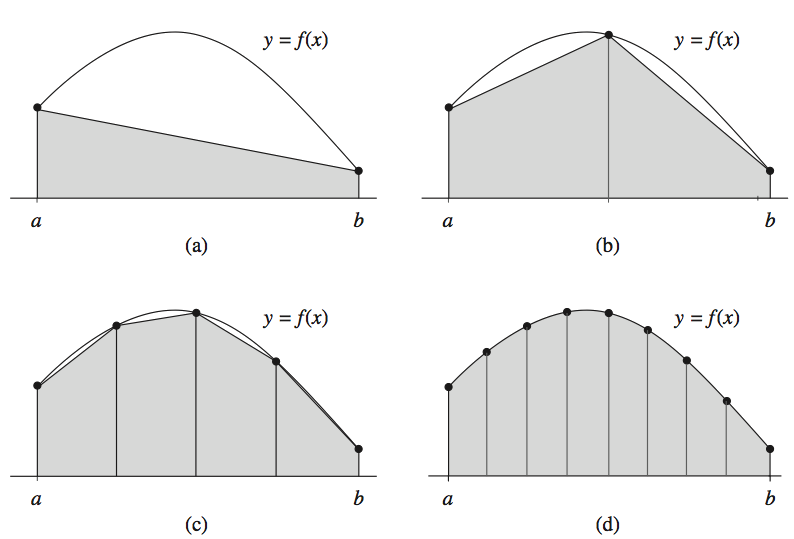
\includegraphics[width=95mm]{chap-5/fig_7-8.png}
\caption{(a) $T(0)$ is the area under $2^0 = 1$ trapezoid. 
(b) $T(1)$ is the area under $2^1 = 2$ trapezoids. 
(c) $T(2)$ is the area under $2^2 = 4$ trapezoids. 
(d) $T(3)$ is the area under $2^3 = 8$ trapezoids.}
\end{center}
\end{figure}
}

\frame{
\begin{block}{Theorem (Successive Trapezoidal Rules).}
Suppose that $J \ge 1$ and the points $\{x_k = a + kh\}$ subdivide $[a,b]$ into $2^J = 2M$ subintervals of equal width $h = (b - a) \slash 2^J$.
The trapezoidal rules $T( f, h)$ and $T( f, 2h)$ obey the relationship
\begin{equation*}
T(f,h) = \frac{T(f,2h)}{2} + h \sum_{k=1}^M f(x_{2k-1})
\end{equation*}
\end{block}
\vspace{3mm}
\begin{block}{Definition (Sequence of Trapezoidal Rules). }
Define $T (0) = (h \slash 2)( f (a) + f (b))$, which is the trapezoidal rule with step size $h = b - a$. 
Then for each $J \ge 1$ define $T(J) = T(f,h)$, where $T(f,h)$ is the trapezoidal rule with step size $h = (b - a) \slash 2^J$.
\end{block}
}

\frame{
\begin{block}{Corollary (Recursive Trapezoidal Rule).} 
Start with $T(0) = (h \slash 2)(j(a) + f(b))$. 
Then a sequence of trapezoidal rules $\{ T(J) \}$ is generated by the recursive formula
\begin{equation*}
T(J) = \frac{T(J-1)}{2} + h \sum_{k=1}^M f(x_{2k-1}) \ \ \ \ \ for \ J = 1,2,\ldots
\end{equation*}
where $h = (b-a)/2^J$ and $\{ x_k = a + kh \}$
\end{block}
Proof: \\
For the even nodes $x_0 < x_2 < \cdots < x_{2M-2} < x_{2M}$, 
we use the trapezoidal rule with step size $2h$:
\begin{equation*}
T(J -1)= \frac{2h}{2} \left( f_0 +2f_2 +2f_4 + \cdots +2f_{2M-4} + 2f_{2M-2} + f_{2M} \right). 
\end{equation*}
\begin{center}
$\Downarrow$
\end{center}
}

\frame{
\frametitle{Proof of Corollary (continue.) }
For all of the nodes $x_0 < x_1 < x_2 < \cdots < x_{2M-1} < x_{2M}$, we use the trapezoidal rule with step size $h$:
\begin{equation*}
T(J)= \frac{h}{2} \left( f_0 +2f_1 +2f_2 + \cdots + 2f_{2M-2} + 2f_{2M-1} + f_{2M} \right). 
\end{equation*}
\begin{center}
$\Downarrow$
\end{center}
Collecting the even and odd subscripts in the above yields
\begin{equation*}
T(J) = \frac{h}{2} \left( f_0 + 2f_2 + \cdots + 2f_{2M-2} + f_{2M} \right) + h \sum_{k=1}^M f_{2k-1}
\end{equation*}
\begin{center}
$\Downarrow$
\end{center}
Substituting $T(J-1)$ into $T(J)$ results in $T ( J ) = T ( J - 1) \slash 2 + h \sum_{k=1}^M f_{2k - 1} $.
}

\frame{
\begin{block}{Example.}
Use the sequential trapezoidal rule to compute the approximations $T(0)$, $T(1)$, $T(2)$, and $T(3)$ for the integral $\int_1^5 d x \slash x = \ln(5) - \ln(1) = 1.609437912$.
\end{block}
The following table shows the nine values required to compute $T(3)$ and the midpoints required to compute $T (1)$, $T (2)$, and $T (3)$. 
\begin{figure}
\begin{center}
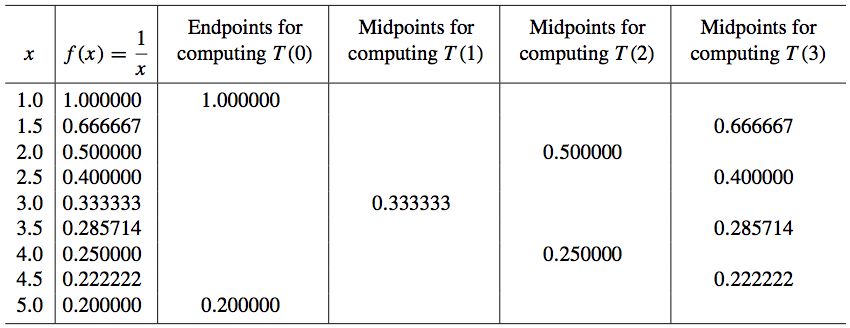
\includegraphics[width=90mm]{chap-5/tab_7-4.png}
\end{center}
\end{figure}
}

\frame{
Details for obtaining the results are as follows:
\begin{itemize}
\item When $h = 4$ :
\begin{equation*}
T(0) = \frac{4}{2} (1.000000 + 0.200000) = 2.400000
\end{equation*}
\item When $h = 2$ :
\begin{equation*}
\begin{array}{l l}
T(1) & = \frac{T(0)}{2} + 2(0.333333) \\
& = 1.200000 + 0.666666 = 1.866666.
\end{array}
\end{equation*}
\item When $h = 1$ :
\begin{equation*}
\begin{array}{l l}
T(2) & = \frac{T(1)}{2} + 1(0.500000 + 0.250000) \\
& = 0.933333 + 0.750000 = 1.683333.
\end{array}
\end{equation*}
\item When $h = \frac{1}{2}$ :
\begin{equation*}
\begin{array}{l l}
T(3) & = \frac{T(2)}{2} + \frac{1}{2} (0.666667 + 0.400000 + 0.285714 + 0.222222) \\
& = 0.841667 + 0.787302 = 1.628968.
\end{array}
\end{equation*}
\end{itemize}
}

\frame{
\begin{block}{Theorem (Recursive Simpson Rules).}
Suppose that $\{T ( J )\}$ is the sequence of trapezoidal rules generated by the above Corollary.
If $J \ge 1$ and $S(J)$ is Simpson’s rule for $2^J$ subintervals of $[a,b]$, 
then $S(J)$ and the trapezoidal rules $T(J-1)$ and $T(J)$ obey the relationship
\begin{equation*}
S(J) = \frac{4T(J) - T(J-1)}{3} \hspace{5mm}  for \ J = 1, 2, \ldots
\end{equation*}
\end{block}
Proof \\
The trapezoidal rule $T(J)$ with step size $h$ yields the approximation
\begin{equation*}
\begin{array}{l l}
\int_a^b f(x) dx & \approx \frac{h}{2} \left( f_0 +2f_1 +2f_2 + \cdots + 2f_{2M-2} +2f_{2M-1} + f_{2M} \right) \\
& \\
& = T(J).
\end{array}
\end{equation*}

}

\frame{
\frametitle{Proof of Theorem (continue) }
The trapezoidal rule $T ( J - 1)$ with step size $2h$ produces
\begin{equation*}
\begin{array}{l l}
\int_a^b f(x) dx & \approx h \left( f_0 +2f_2 + \cdots + 2f_{2M-2} + 2f_{2M-1} + f_{2M} \right) \\
& \\
& = T(J-1).
\end{array}
\end{equation*}
\begin{center}
$\Downarrow$
\end{center}
Multiplying relation of first equation by 4 yields
\begin{equation*}
\begin{array}{l l}
4 \int_a^b f(x) dx & \approx h \left( 2f_0 + 4f_1 +4f_2 + \cdots + 4f_{2M-2} + 4f_{2M-1} + 2f_{2M} \right) \\
& \\
& =4 T(J).
\end{array}
\end{equation*}
\begin{center}
$\Downarrow$
\end{center}
Now subtract $\int_a^b f(x) dx$ from $4 \int_a^b f(x) dx$ and the result is 
\begin{equation*}
\begin{array}{l l}
3 \int_a^b f(x) dx & \approx h \left( f_0 + 4f_1 +4f_2 + \cdots + 4f_{2M-2} + 4f_{2M-1} + f_{2M} \right) \\
& \\
& =4 T(J) - T(J-1).
\end{array}
\end{equation*}
}

\frame{
\frametitle{Proof of Theorem (continue) }
\begin{center}
$\Downarrow$
\end{center}
This can be rearranged to obtain
\begin{equation*}
\begin{array}{l l}
\int_a^b f(x) dx & \approx \frac{h}{3} \left( f_0 + 4f_1 +4f_2 + \cdots + 4f_{2M-2} + 4f_{2M-1} + f_{2M} \right) \\
& \\
& = \frac{4 T(J) - T(J-1)}{3} .
\end{array}
\end{equation*}
The middle term is Simpson's rule $S(J) = S(f, h)$ and hence the theorem is proved. 
\begin{center}
$\Downarrow$
\end{center}
\begin{equation*}
S(J) = \frac{4T(J) - T(J-1)}{3} \hspace{5mm}  for \ J = 1, 2, \ldots
\end{equation*}
}

\frame{
\begin{block}{Example.}
Use the sequential Simpson rule to compute the approximations $S(1)$, $S(2)$, and $S(3)$ for the integral.
\end{block}
Using the results of the above example:  $T(0)$, $T(1)$, $T(2)$, and $T(3)$ with J = 1, 2, and 3, we compute
\begin{equation*}
\begin{array}{l l l l}
S(1) & = \frac{4T(1)-T(0)}{3} & = \frac{4(1.866666) - 2.400000}{3} & = 1.688888 \\
& & & \\
S(2) & = \frac{4T(2)-T(1)}{3} & = \frac{4(1.683333) - 1.866666}{3} & = 1.622222 \\
& & & \\
S(3) & = \frac{4T(3)-T(2)}{3} & = \frac{4(1.628968) - 1.683333}{3} & = 1.610846
\end{array}
\end{equation*}
}

\frame{
\frametitle{the Sequential Boole and Simpson rules}
It was obtained by integrating the Lagrange polynomial of degree 4 based on the nodes $x_0$, $x_1$, $x_2$, $x_3$, and $x_4$. 
\vspace{5mm}
\begin{center}
$\Downarrow$
\end{center}
\vspace{5mm}
\begin{block}{}
When it is applied $M$ times over $4M$ equally spaced subintervals of $[a, b]$ of step size $h = (b - a) \slash (4M)$, 
we call it the {\Large composite Boole rule}:
\begin{equation*}
B(f,h) = \frac{2h}{45} \sum_{k=1}^{M} \left( 7f_{4k-4} +32f_{4k-3} +12f_{4k-2} +32f_{4k-1} +7f_{4k} \right)
\end{equation*}
\end{block}
}

\frame{
\begin{block}{Theorem (Recursive Boole Rules).}
Suppose that $\{ S(J) \}$ is the sequence of Simpson’s rules generated by Theorem  of the Recursive Simpson Rules. \\
\vspace{3mm}
If $J \ge 2$ and $B(J)$ is Boole’s rule for $2^J$ subintervals of $[a,b]$,  \\
\begin{center}
$\Downarrow$
\end{center}
then $B(J)$ and Simpson’s rules $S(J - 1)$ and $S(J)$ obey the relationship
\vspace{3mm}
\begin{equation*}
B(J) = \frac{16S(J) - S(J-1)}{15} \ \ for \ \ J = 2, 3, \ldots
\end{equation*}
\end{block}
}

\frame{
\begin{block}{Example.}
Use the sequential Boole rule to compute the approximations $B(2)$ and $B(3)$ for the integral of the above Example.
\end{block}
Using the results of the above example : $S(1)$, $S(2)$, and $S(3)$ with J = 2 and 3, we compute
\begin{equation*}
\begin{array}{l l l l}
B(2) & = \frac{16S(2) - S(1)}{15} & = \frac{16(1.622222) - 1.688888}{15}  & = 1.617778\\
& & & \\
B(3) & = \frac{16S(3) - S(2)}{15} & = \frac{16(1.610846) - 1.622222}{15}  & = 1.610088
\end{array}
\end{equation*}
The next level of approximation\footnote{an accuracy of five decimal places.} for the integral is
\begin{equation*}
\frac{64B(3) - B(2)}{63} = \frac{64(1.610088)}{63} = 1.609490
\end{equation*}
}

\frame{
\frametitle{Romberg Integration}
The error terms $E_T(f, h)$ and $E_S(f, h)$ for the composite trapezoidal rule and composite Simpson rule are of order $O(h^2)$ and $O(h^4)$, respectively. 
\begin{center}
$\Downarrow$
\end{center}
It is not difficult to show that the error term $E_B(f, h)$ for the composite Boole rule is of the order $O(h^6)$. 
\begin{center}
$\Downarrow$
\end{center}
\begin{block}{}
\begin{equation*}
\begin{array}{l l}
\int_a^b f(x) dx & = T(f,h)+ O(h^2)\\
& \\
\int_a^b f(x) dx & = S(f,h)+ O(h^4) \\
& \\
\int_a^b f(x) dx & = B(f,h)+ O(h^6) \\
\end{array}
\end{equation*}
\end{block}
}

\frame{
\begin{itemize}
\item Suppose that an approximation rule is used with step sizes $h$ and $2h$; then an algebraic manipulation of the two answers is used to produce an improved answer. 
\item Each successive level of improvement increases the order of the error term from $O(h^{2N})$ to $O(h^{2N+2})$. 
\end{itemize}
\begin{center}
$\Downarrow$
\end{center}
\begin{block}{}
This process, called {\Large Romberg integration}, has its strengths and weaknesses. 
\end{block}
}

\frame{
\begin{block}{}
The Newton-Cotes rules are seldom used past Boole's rule. 
\end{block}
\begin{itemize}
\item This is because the nine-point Newton-Cotes quadrature rule involves negative weights, and all the rules past the 10-point rule involve {\Large negative weights}. 
\vspace{0.3cm}
\item This could introduce loss of significance error due to round off. 
\vspace{0.3cm}
\end{itemize}
\begin{block}{}
The {\Large Romberg method} has the advantages that all the weights are {\Large positive} and the equally spaced abscissas are easy to compute. 
\end{block}
}

\frame{
 A computational weakness of Romberg integration is that twice as many function evaluations are needed to decrease the error from $O(h^{2N})$ to $O(h^{2N+2})$. 
\begin{center}
$\Downarrow$
\end{center}
The development of  Romberg integration relies on the theoretical assumption that, if $f \in C^N[a, b]$ for all $N$, then the error term for the trapezoidal rule can be represented in a series involving only even powers of $h$; that is, 
\begin{block}{}
\begin{equation*}
\int_a^b f(x) d x = T (f, h) + E_T (f, h)
\end{equation*}
where 
\begin{equation*}
E_T (f, h) = a_1 h^2 + a_2 h^4 + a_3 h^6 + \cdots
\end{equation*}
\end{block}
}

\frame{
Since only even powers of $h$ can occur in $\int_a^b f(x) d x $, the Richardson improvement process is used successively first to eliminate $a_1$, next to eliminate $a_2$, then to eliminate $a_3$, and so on.  \\
This process generates quadrature formulas whose error terms have even orders $O(h^4)$, $O(h^6)$, $O(h^8)$, and so on. 
\begin{center}
$\Downarrow$
\end{center}
We shall show that the first improvement is Simpson's rule for $2M$ intervals.  \\
Start with $T(f, 2h)$ and $T(f, h)$ and the equations 
\begin{center}
$\Downarrow$
\end{center}
\begin{equation*}
\int_a^b f(x) dx = T(f, 2h) + a_1 4 h^2 + a_2 16 h^4 + a_3 64 h^6 + \cdots
\end{equation*}
and
\begin{equation*}
\int_a^b f(x) dx = T(f, h) + a_1 h^2 + a_2 h^4 + a_3 h^6 + \cdots
\end{equation*}
}

\frame{
Multiply equation $\int_a^b f(x) d x $ by $4$ and obtain 
\begin{equation*}
4 \int_a^b f(x) dx = T(f, h) + a_1 4 h^2 + a_2 4 h^4 + a_3 4 h^6 + \cdots
\end{equation*}
\begin{center}
$\Downarrow$
\end{center}
Eliminate $a_1$ by subtracting $\int_a^b f(x) d x $ from $4 \int_a^b f(x) d x $. 
The result is 
\begin{equation*}
3 \int_a^b f(x) dx = 4 T(f, h) - T(f, 2h) - a_2 12 h^4 - a_3 60 h^6 - \cdots
\end{equation*}
\begin{center}
$\Downarrow$
\end{center}
Now divide equation $3 \int_a^b f(x) d x $ by $3$ and rename the coefficients in the series:
\begin{equation*}
\int_a^b f(x) dx = \frac{4 T(f, h) - T(f, 2h)}{3} + b_1 h^4 + b_2 h^6 - \cdots
\end{equation*}
}

\frame{
The first quantity on the right side of $\int_a^b f(x) d x $ is Simpson's rule $S(f, h)$. 
This shows that $E_S(f, h)$ involves only even powers of $h$: 
\begin{equation*}
\int_a^b f(x) dx = S(f, h) + b_1 h^4 + b_2 h^6 + b_3 h^8 + \cdots
\end{equation*}
\begin{center}
$\Downarrow$
\end{center}
To show that the second improvement is Boole's rule,  write down the formula involving $S(f, 2h)$: 
\begin{equation*}
\int_a^b f(x) dx = S(f, 2h) + b_1 16 h^4 + b_2 64 h^6 + b_3 256 h^8 + \cdots
\end{equation*}
\begin{center}
$\Downarrow$
\end{center}
When $b_1$ is eliminated, the result involves Boole's rule: 
\begin{equation*}
\begin{array}{l l}
\int_a^b f(x) dx & =  - \frac{16S( f, h) - S( f, 2h)}{15}  - \frac{b_2 48 h^6}{15}  - \frac{b_3 240 h^8}{15} + \cdots \\
& = B(f, h) - \frac{b_2 48 h^6}{15} - \frac{b_3 240 h^8}{15} - \cdots
\end{array}
\end{equation*}
}

\frame{
\begin{block}{Lemma (Richardson’s Improvement for Romberg Integration).}
Given two approximations $R(2h, K - 1)$ and $R(h, K - 1)$ for the quantity $Q$ that satisfy
\begin{equation*}
Q = R(h,K -1) + c_1 h^{2K} + c_2h^{2K+2} + \cdots
\end{equation*}
and
\begin{equation*} 
Q = R(2h,K -1) + c_1 4^K h^{2K} + c_2 4^{K+1} h^{2K+2} + \cdots ,
\end{equation*}
an improved approximation has the form
\begin{equation*} 
Q = \frac{4^K R(h, K-1) - R(2h, K-1)}{4^K - 1} + O(h^{2K+2})
\end{equation*}
\end{block}
}

\frame{
\begin{block}{Definition}
Define the sequence $\{ R(J, K) : J ≥ K\}_{J=0}^\infty$ of quadrature formulas for $f (x)$ over $[a, b]$ as follows:
\begin{itemize}
\item $R(J,0) = T(J)$   for $J \ge 0$, is the sequential trapezoidal rule.
\item $R(J,1) = S(J)$   for $J \ge 1$, is the sequential Simpson rule.
\item $R(J,2) = B(J)$   for $J \ge 2$, is the sequential Boole’s rule.
\end{itemize}
\end{block}
\vspace{0.5cm}
The starting rules, 
$\{R(J, 0)\}$, are used to generate the first improvement, 
$\{R(J, 1)\}$, which in turn is used to generate the second improvement, $\{R(J, 2)\}$. 
}

\frame{
We have already seen the patterns
\begin{equation*}
\begin{array}{l l l}
R(J,1) & = \frac{4^1 R(J,0) - R(J-1,0)}{4^1 -1} & for \ \ J \ge 1 \\
& & \\
R(J,2) & = \frac{4^2 R(J,1) - R(J-1,1)}{4^2 -1} & for \ \ J \ge 2 
\end{array}
\end{equation*}
The general rule for constructing improvements is
\begin{equation*}
R(J, K) = \frac{4^K R(J,K-1)-R(J-1,K-1)}{4^K - 1} \ \ for \  J \ge K
\end{equation*}
}

\frame{
For computational purposes, the values $R(J, K)$ are arranged in the Romberg integration tableau : 
\begin{figure}
\begin{center}
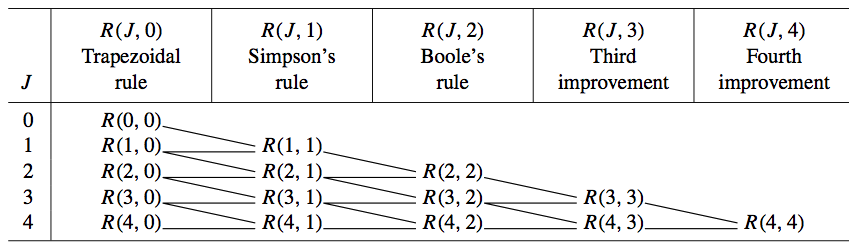
\includegraphics[width=100mm]{chap-5/tab_7-5.png}
\end{center}
\end{figure}
}

\frame{
\begin{block}{Example.}
Use Romberg integration to find approximations for the definite integral
\begin{equation*}
\int_0^{\Pi \slash 2} \left( x^2 + x + 1\right) \cos (x) dx = -2 + \frac{\Pi}{2} + \frac{\Pi^2}{4} = 2.038197427067\ldots 
\end{equation*}
\end{block}
The computations are given in the following table. 
\begin{figure}
\begin{center}
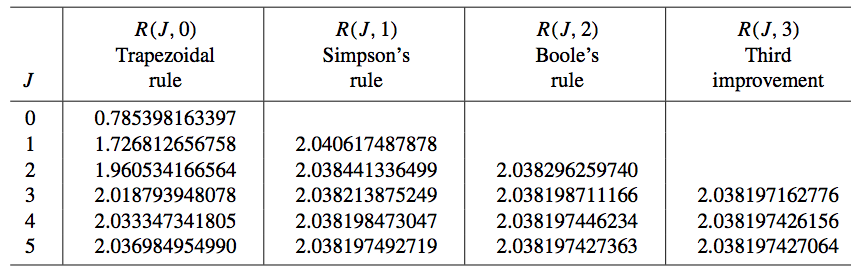
\includegraphics[width=100mm]{chap-5/tab_7-6.png}
\end{center}
\end{figure}
}

\frame{
In each column the numbers are converging to the value $2.038197427067 \ldots$. 
\begin{itemize}
\item  The values in the Simpson's rule column converge faster than the values in the trapezoidal rule column. 
\item  For this example, convergence in columns to the right is faster than the adjacent column to the left. 
\end{itemize}
\begin{figure}
\begin{center}
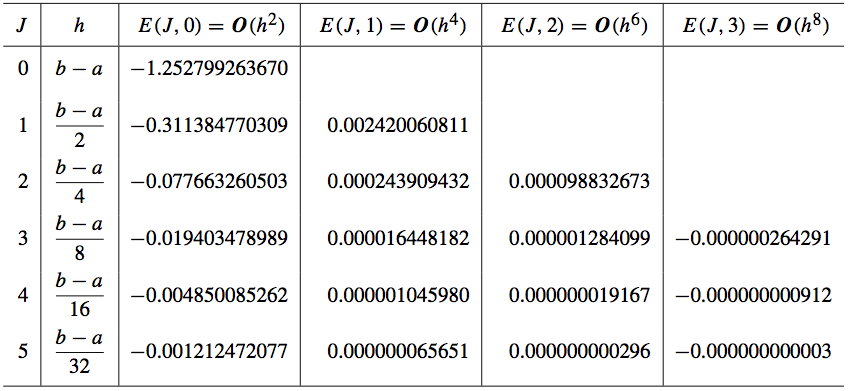
\includegraphics[width=100mm]{chap-5/tab_7-7.png}
\end{center}
\end{figure}
}

\frame{
\begin{itemize}
\item Convergence of the Romberg values in the above Table  is easier to see if we look at the error terms $E( J, K) = -2 + \pi / 2 + \pi^2 / 4 - R( J, K)$. 
\vspace{3mm}
\item Suppose that the interval width is $h = b - a$ and that the higher derivatives of $f(x)$ are of the same magnitude. 
\vspace{3mm}
\item The error in column $K$ of the Romberg table diminishes by about a factor of $1/2^{2K+2} = 1/4^{K+1}$ as one progresses down its rows. 
\vspace{3mm}
\item The errors $E(J, 0)$ diminish by a factor of $1/4$, the errors $E(J, 1)$ diminish by a factor of $1/16$, and so on. 
\end{itemize}
}

\frame{
\begin{block}{Theorem (Precision of Romberg Integration).}
Assume that $f \in C^{2K+2}[a,b]$. 
Then the truncation error term for the Romberg approximation is given in the formula
\begin{equation*}
\begin{array}{l l}
\int_a^b f(x) dx & = R(J,K) + b_K h^{2K+2} f^{(2K+2)} (c_J,K) \\
& = R(J,K) + O(h^{2K+2})
\end{array}
\end{equation*}
where $h =(b-a) \slash 2^J$, $b_K$ is a constant that depends on $K$, and $c_{J,K} \in [a,b]$.
\end{block}
}

\frame{
\begin{block}{Example.}
Apply Theorem of Precision of Romberg Integration and show that
\begin{equation*}
\int_0^2 10 x^9 dx = 1024 \equiv R(4,4).
\end{equation*}
\end{block}
\vspace{0.3cm}
The integrand is $f (x) = 10 x^9$, and $f (10)(x) \equiv 0$. 
\begin{center}
$\Downarrow$
\end{center}
Thus the value $K = 4$ will make the error term identically zero. 
\begin{center}
$\Downarrow$
\end{center}
A numerical computation will produce $R(4, 4) = 1024$.
}

